\chapter{Heart Sound Segmentation}

\section{Introduction}

In this subsystem, the aim is to pre-process the PCG data, measured by the microphones, so that it can be used by the localization system. The localization system requires its input data to be an audio segment where only S1 segments are present (S2 segments and silent parts removed), and an audio segment with only S2 segments.

To achieve this, the following steps have been taken:
\begin{enumerate}
    \item \textbf{Preprocessing}: The signal was prepared for ease of processing.
    \item \textbf{Detection}: The location of the S1 and S2 sounds in the sound file was retrieved.
    \item \textbf{Segmentation}: The recorded sound is cut up into S1 and S2 sounds.
\end{enumerate}

To achieve this, it is necessary to detect where the wanted sounds are and to isolate them. It is important that the sound signals that do not belong to an S1 or S2 sound are not selected, as that would result in faulty data. Moreover, S1 or S2 sounds should not be skipped, as this would result in excluding data that could be necessary and might have an influence on the detection of surrounding peaks. Another challenge is distinguishing S1 sounds from S2 sounds, as they have to be separated from each other. A possibility is to look at the timing of the peaks, using the knowledge that they originate from four different heart valves closing at two different time intervals.


\section{Preprocessing}
For the analysis of the heart sounds, not all frequencies in the signal are relevant. Therefore, a bandpass filter with cut-off frequencies of 10 Hz and 800 Hz was applied to the signals. After that, because the input signals are sampled at 48 kHz, the signals were downsampled to 4 kHz, to ensure quicker processing. Following that, the signals were normalized to a maximum height of 1, and converted to an energy signal using the Shannon Energy formula:

\begin{equation}
    \label{eq:shannonenergy}
    E(t) = - x_n^2(t) log(x_n^2(t))
\end{equation}

This signal was then normalized in a way that ensure that the standard deviation is 1. Following that, a lowpass filter with a cut-off frequency of 7 Hz was applied, to smoothen out the energy, which is beneficial for following processing steps. The signal that is present after all of the steps until now have been taken will be referred to as the Shannon Energy Envelope, or SEE in short.


\section{Detection}
\subsection{Peak detection}
To detect the S1 and S2 peaks, a threshold based peak detection on the SEE was used, with a threshold set at 30\% of the standard deviation, and a minimum distance between peaks set to be 0.23 seconds. These parameters prevent too many peak being detected, whilst also ensuring not to skip too many. All peaks that this algorithm detects are candidates to be either an S1 or an S2 peak. 
\subsection{Time differences of peaks}
To check if the detected peaks are correct, the locations of the peaks were analyzed. Only the time axis of the locations  were analyzed, as the height of the peaks can differ greatly between heart beats, and is therefore not a consistent measure. 
The time differences between the peaks were calculated, which is used in the following steps to classify the peaks as either an S1, S2 or an uncertain peak.
\subsection{Classification}
As the time between an S1 peak and an S2 peak of the same heartbeat is almost always shorter than the time between an S2 peak and the S1 peak of the next heartbeat, the graph of the time differences should alternate between a maxima and minima (as seen in Fig. \ref{fig:differences} everywhere except between t=8s and t=10s). However, as sometimes there are maxima lower than certain minima, and some differences are neither a maximum or a minimum, it is necessary to base the detection on a vertical threshold, which is lower than most maxima and higher than most minima. A peak was then labeled as an S1 peak if the time difference was lower than the threshold and the previous peak was \textbf{not} an S1 peak. A peak was labeled as an S2 peak if the time difference was higher than the threshold and the previous peak was \textbf{not} an S2 peak. If neither of these conditions satisfy, the peak is labeled as an uncertain peak. Peaks were also labeled as uncertain in case they came earlier than 200ms after a previous peak, as a systole of a human heart has a minimum length of 200ms \cite{systole_length}, and the diastole is assumed to always be longer than the systole.

\begin{figure} [H]
    \centering
    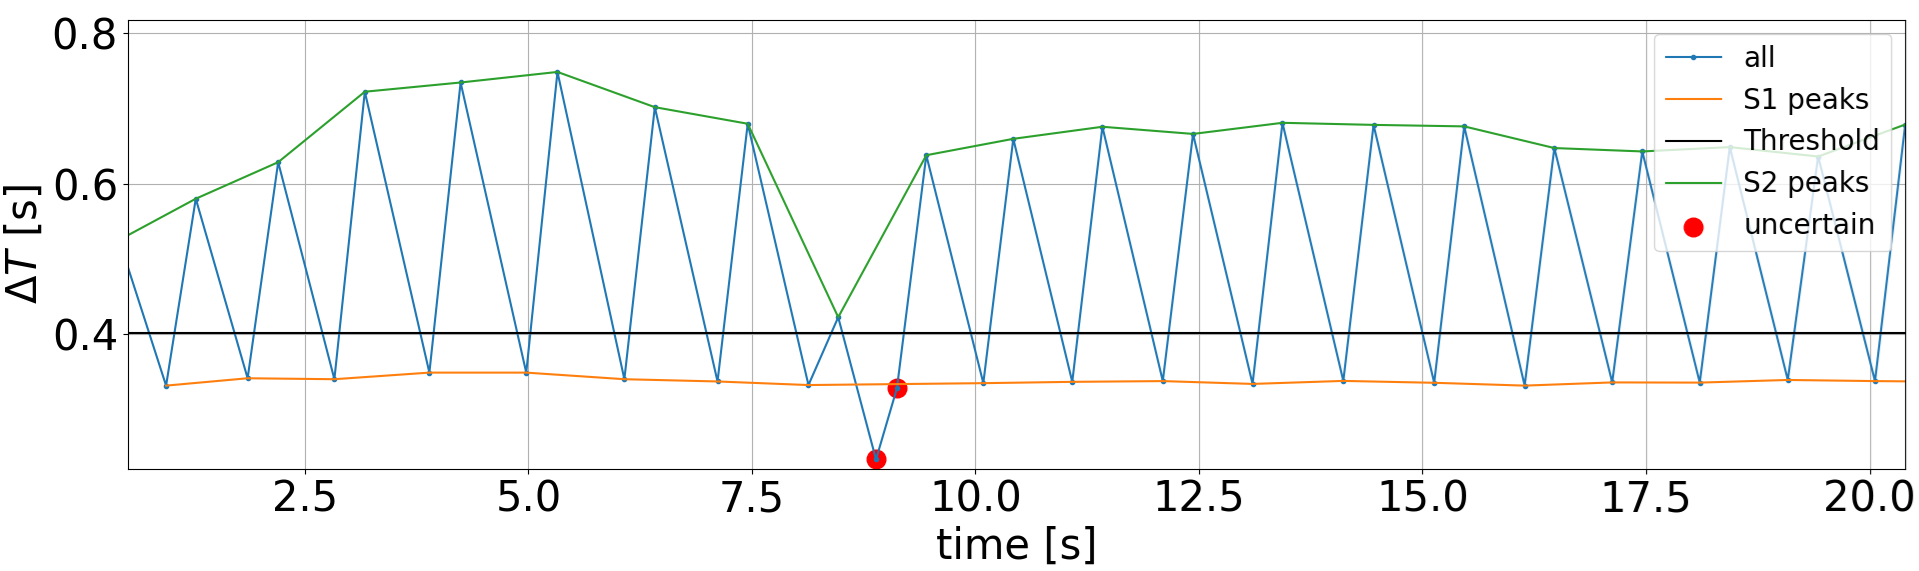
\includegraphics[width=0.9\textwidth]{docs/assignments/Final report/figures/module_1/differences.png}
    \caption{Time differences between detected peaks of a measured heartbeat, including first classification of peaks.}  
    \label{fig:differences}
\end{figure}

\subsection{Solve uncertain peaks}
In case there are more uncertain peaks than a predefined number of uncertain peaks per minute that are allowed, a method has been implemented to try and resolve these uncertain peaks. It is assumed that in the vicinity of the uncertain peaks there has been detected a peak too much or a peak too little, which means that a peak has to be removed (which is not necessarily the uncertain peak itself) or a peak has to be added. It is determined if there is either a peak too much or a peak too little detected by comparing the time difference of the uncertain peak to the threshold: if it is higher than the threshold, there has likely been a peak too little detected, and if it is lower than the threshold, there has likely been a peak too much detected. To resolve this, the peak detection threshold is adjusted in two ways. 

Firstly, the peak detection threshold is adjusted for the whole signal, by increasing it if too many peaks have been detected and decreasing it if too little peaks have been detected. After that all peaks are reclassified using the same method as used before. This is continued until either enough uncertain peaks have been resolved, or either a maximum adjustment has been reached.

Secondly, if adjusting the peak detection threshold across the whole signal does not result in little enough uncertain peaks, the threshold is also adjusted locally. This is done as heartbeat can differ greatly, so local detection could be necessary. This was achieved by considering uncertain peaks that occur sequentially as one group. For each group, the peak detection is adjusted (either up or down according too either too many or too little peaks), and only the difference in detected peaks on the interval of the uncertain group is updated. All peaks of the whole signal are then reclassified. This is continued until there are no uncertain peaks left in the group, or a maximum adjustment has been reached.


\section{Segmentation}
The goal of segmentation is to cut out the S1 and S2 parts of the signal. This is done by using a relatively low threshold on the SEE to detect peaks. The intersections of the SEE and the threshold are also acquired. The locations of the S1 and S2 peaks are then used to determine which intervals of intersections should be used to segment the signal: if a peak is in between two intersections, those intersections mark the interval on which the S1 or S2 peak occurs. 

\section{Integration}
For further systems, it is necessary to provide the original PCG signals of only the S1 or S2 peaks. As the intervals of the segments currently obtained are based on signals which have a sample rate of 4kHz, the bounds of the intervals were upscaled to correspond to the correct intervals in the original PCG signals, which has a sample rate of 48kHz. The parts that were cut out in this way were concatenated together, resulting in a signal consisting of only S1 or S2 peaks. 


\section{Testing}

The system was first tested on the simulated data of the model described in the previous chapter. This resulted in the data presented in Fig. \ref{fig:segmented_model}. All peaks seem to been detected correctly. The randomization effect of the model is also visible, as the peaks don't all have the same height and the time differences between the peaks are not all the same, which would be the case if every heartbeat were identical. The peak heights do seem to differ more than the peaks of a real heartbeat would, which could mean that the randomization is too strong.

\begin{figure} [H]
    \centering
    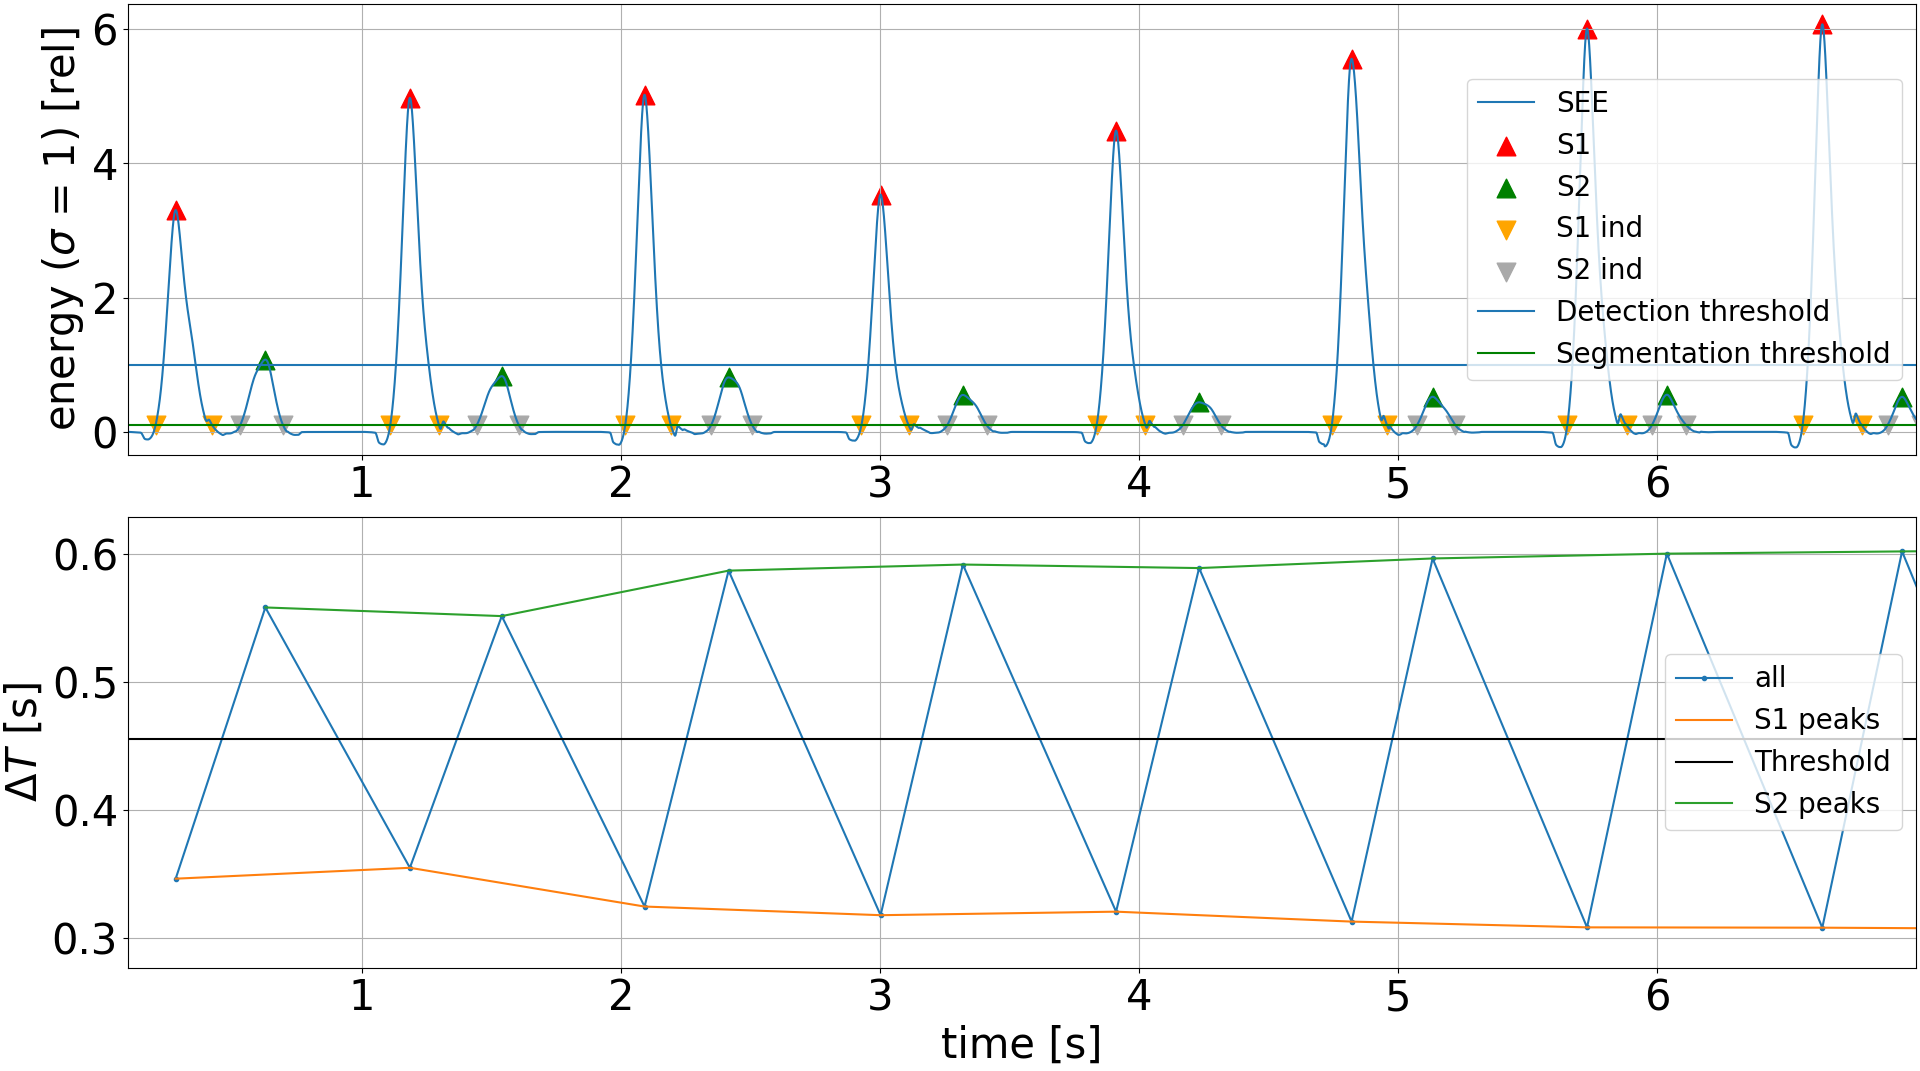
\includegraphics[width=0.95\textwidth]{docs/assignments/Final report/figures/module_1/model_segmented.png}
    \caption{SEE and time differences of peaks of a modeled heartbeat.}  
    \label{fig:segmented_model}
\end{figure}


Fig. \ref{fig:solveduncertains} shows the same signal as in Fig. \ref{fig:differences}, after also solving the uncertain peaks around t = 9s and zooming in on them. It is apparent that the small peak just before t = 9s has been discarded, and the peak right after has been marked as an S1 peak. This seems to be the right choice, however we aren't trained professionals, and therefore aren't as credible as individuals who are.
\newline The segmentation has also been shown in the SEE plot, which correctly mark the begin and end of assumed S1 and S2 peaks.


\begin{figure} [H]
    \centering
    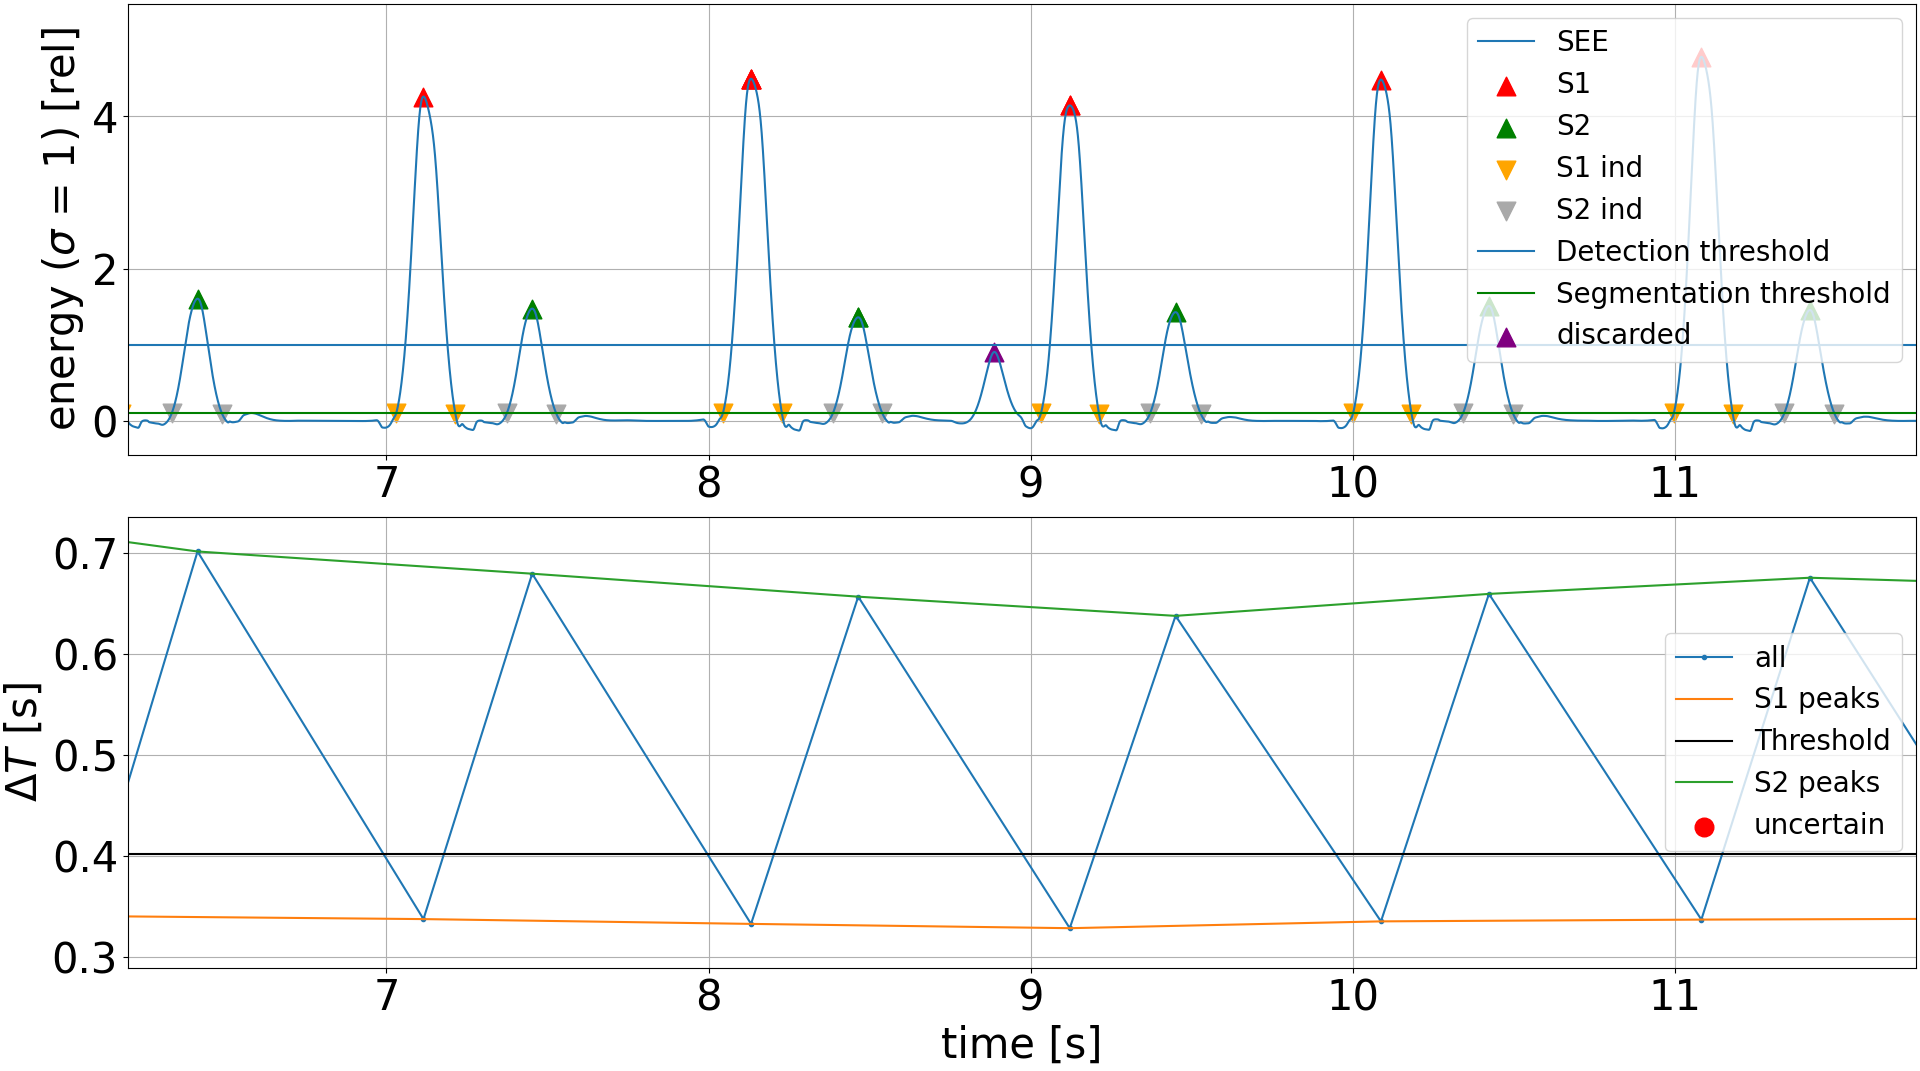
\includegraphics[width=0.95\textwidth]{docs/assignments/Final report/figures/module_1/solved_uncertain.png}
    \caption{SEE and time differences of peaks of same signal as Fig. \ref{fig:differences}, after uncertain peaks have been resolved.}  
    \label{fig:solveduncertains}
\end{figure}

Fig. \ref{fig:failures} shows the SEE and time differences of a different signal. In this case, the uncertain peaks between t = 6s and t = 8s couldn't be resolved. This is likely due to there being two small peaks at the location of where the S2 peak should probably be. However, before t = 6s and after t = 8s, the S2 peaks do seem to be classified correctly. it can also be noted that the detection threshold is equal to 1. This is because initially too many peaks were detected, after which the threshold was increased. This however didn't solve enough uncertain peaks, which is why it stopped at exactly 1, which was the maximum adjustment that was set. The S2 peaks that have been detected correctly therefore have to be detected by the local threshold adjustment, which seems to work in most cases.


\begin{figure} [H]
    \centering
    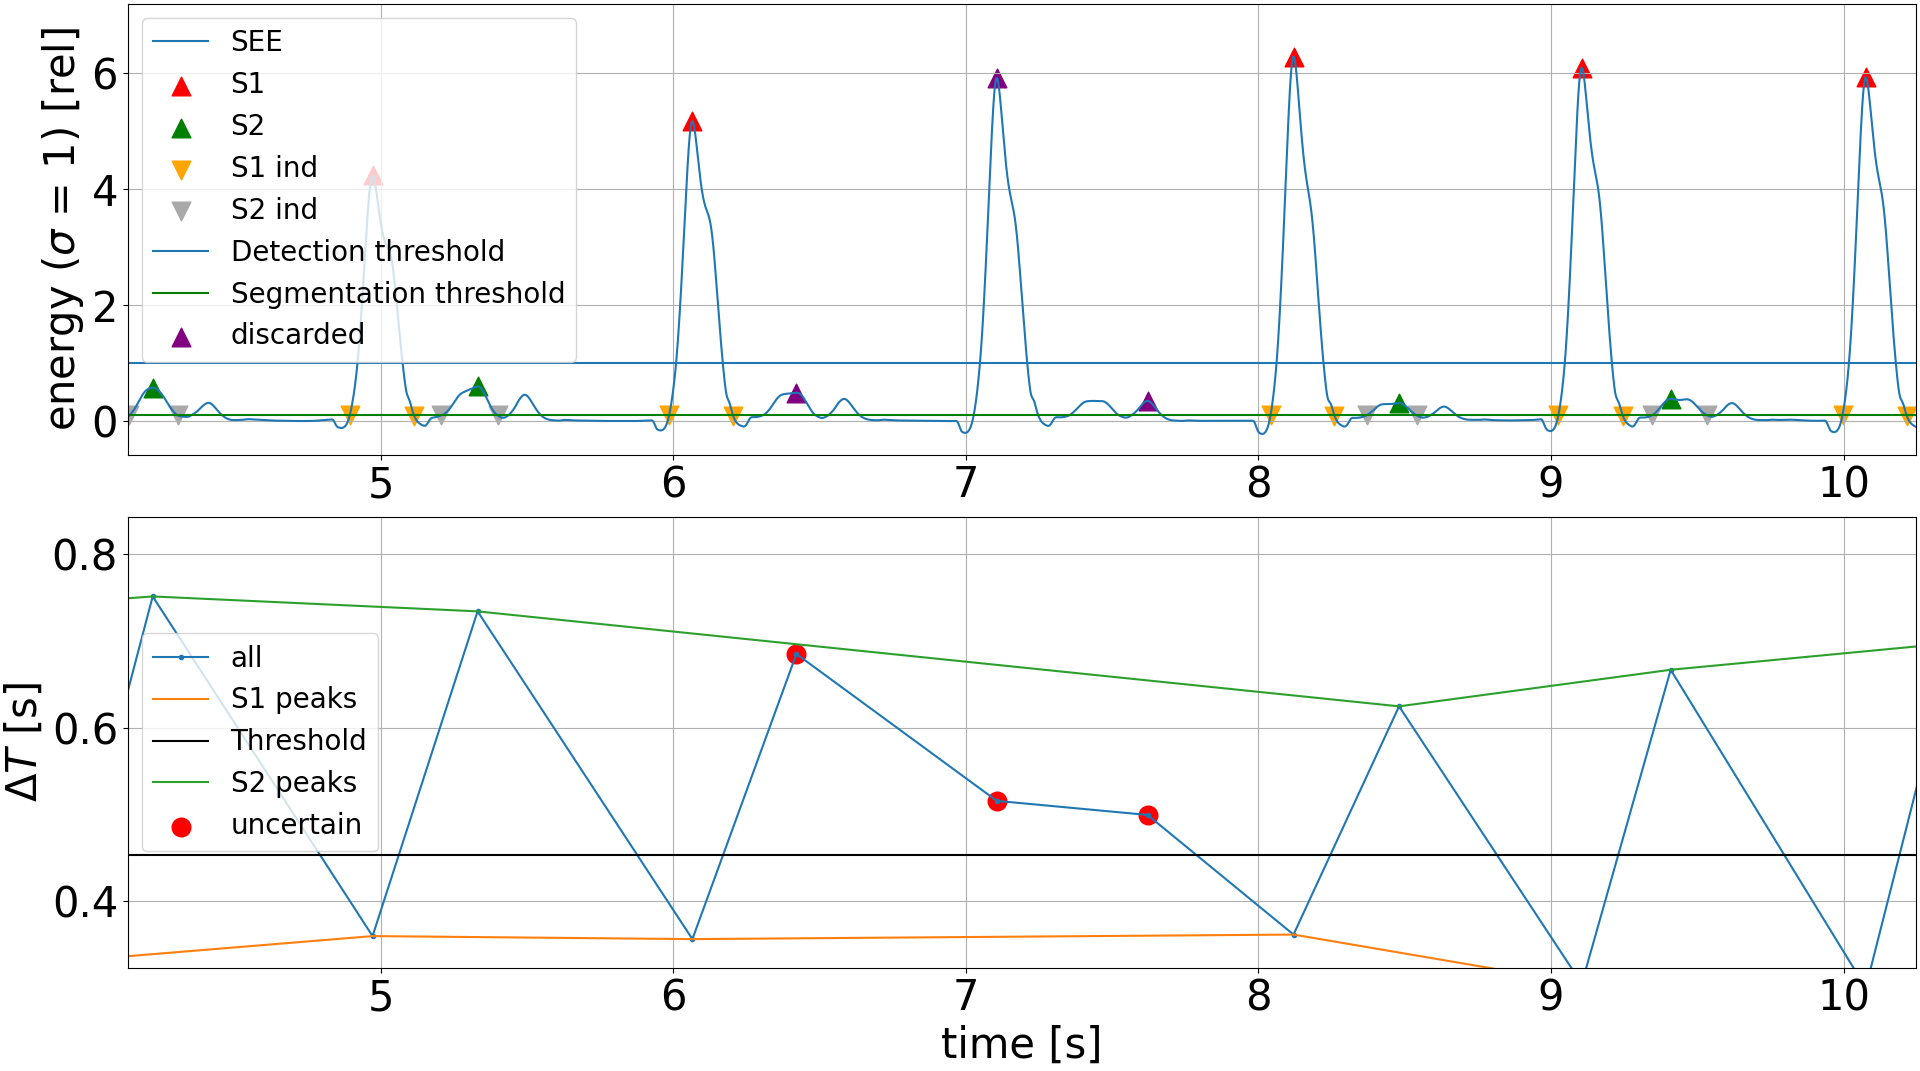
\includegraphics[width=0.95\textwidth]{docs/assignments/Final report/figures/module_1/failures.png}
    \caption{SEE and time differences of peaks, after uncertain peaks have not correctly been resolved.}  
    \label{fig:failures}
\end{figure}

The accuracy of the system was tested on 4 sets of signals: 2 acquired by using stethoscopes and 2 acquired by using piezo electric instrumentation. Each set has 6 signal channels (one for each microphone in the microphone array), so in total the system was tested on 24 signals. The signals were checked by visual inspection. Because we are not trained professionals, this implies that what was assumed to be the correct labeling of the peaks might not be correct. It was only checked whether false positives or false negatives occurred. More precise would be to test if the peaks were segmented correctly, however, this is impossible to do by visual inspection. Table \ref{tab:test_piezo_segmentation} and Table \ref{tab:test_stethoscope_segmentation} show the results of the tests. These have been summarized in Table \ref{tab:piezo_results} and Table \ref{tab:stethoscope_results}. In this summary the recordings "Piezo 2 Ch. 6", "Piezo 4 Ch. 4" and "Piezo 4 Ch. 6" have been omitted, as the system detected too many uncertain peaks which resulted in the system crashing. 



\begin{table}[H]
\scriptsize
\centering
\captionsetup{justification=centering}
\begin{tabular}{|l|c|c|c|c|c|c|c|c|c|c|}
\hline
\textbf{Recording} & \textbf{Ch.} & \textbf{S1} & \textbf{S2} & \textbf{Uncertain} &
\multicolumn{2}{c|}{\textbf{False positive}} &
\multicolumn{2}{c|}{\textbf{False negative}} &
\multicolumn{2}{c|}{\textbf{Marked wrong}} \\
\cline{6-11}
 &  &  &  &  & S1 & S2 & S1 & S2 & S1 (is S2) & S2 (is S1) \\
\hline
Piezo 2 & 1 & 120 & 104 & 20 & 1 & 0 & 8 & 8 & 0 & 0 \\
Piezo 2 & 2 & 109 & 90 & 21 & 0 & 1 & 10 & 15 & 0 & 0 \\
Piezo 2 & 3 & 104 & 103 & 2 & 0 & 0 & 0 & 0 & 0 & 0 \\
Piezo 2 & 4 & 95 & 93 & 12 & 0 & 0 & 4 & 8 & 0 & 0 \\
Piezo 2 & 5 & 100 & 100 & 0 & 0 & 0 & 0 & 0 & 0 & 0 \\
\rowcolor{red!30}Piezo 2 & 6 & -- & -- & -- & 0 & 0 & 0 & 0 & 0 & 0 \\
\noalign{\hrule height 0.3pt}
Piezo 4 & 1 & 108 & 104 & 6 & 0 & 0 & 1 & 2 & 0 & 0 \\
Piezo 4 & 2 & 106 & 98 & 19 & 0 & 0 & 4 & 4 & 0 & 0 \\
Piezo 4 & 3 & 102 & 102 & 0 & 0 & 0 & 0 & 0 & 0 & 0 \\
\rowcolor{red!30}Piezo 4 & 4 & -- & -- & -- & 0 & 0 & 0 & 0 & 0 & 0 \\
Piezo 4 & 5 & 102 & 102 & 0 & 0 & 0 & 0 & 0 & 0 & 0 \\
\rowcolor{red!30}Piezo 4 & 6 & 24 & 19 & 83 & 0 & 0 & 78 & 78 & 0 & 0 \\
\hline
\textbf{Total} & & \textbf{946} & \textbf{896} & \textbf{80} &
\textbf{1} & \textbf{1} &
\textbf{27} & \textbf{37} &
\textbf{0} & \textbf{0} \\
\hline
\end{tabular}
\caption{Peak detection evaluation results for the piezo element. Rows colored red contain data the algorithm errored on. On those audio segments, a human eye could only -with great difficulty- detect the peaks and are therefore taken out of the total calculation.}
\label{tab:test_piezo_segmentation}
\end{table}

\begin{table}[H]
\scriptsize
\centering
\captionsetup{justification=centering}
\begin{tabular}{|l|c|c|c|c|c|c|c|c|c|c|}
\hline
\textbf{Recording} & \textbf{Ch.} & \textbf{S1} & \textbf{S2} & \textbf{Uncertain} &
\multicolumn{2}{c|}{\textbf{False positive}} &
\multicolumn{2}{c|}{\textbf{False negative}} &
\multicolumn{2}{c|}{\textbf{Marked wrong}} \\
\cline{6-11}
 &  &  &  &  & S1 & S2 & S1 & S2 & S1 (is S2) & S2 (is S1) \\
\hline
Stethoscope 2 & 1 & 111 & 110 & 0 & 0 & 0 & 0 & 0 & 0 & 0 \\
Stethoscope 2 & 2 & 110 & 109 & 2 & 0 & 0 & 1 & 2 & 0 & 0 \\
Stethoscope 2 & 3 & 111 & 110 & 0 & 0 & 0 & 0 & 0 & 0 & 0 \\
Stethoscope 2 & 4 & 111 & 110 & 0 & 0 & 0 & 0 & 0 & 0 & 0 \\
Stethoscope 2 & 5 & 111 & 110 & 0 & 0 & 0 & 0 & 0 & 0 & 0 \\
Stethoscope 2 & 6 & 111 & 110 & 2 & 0 & 0 & 1 & 1 & 0 & 0 \\
\noalign{\hrule height 0.3pt}
Stethoscope 5 & 1 & 113 & 112 & 0 & 0 & 0 & 0 & 0 & 0 & 0 \\
Stethoscope 5 & 2 & 114 & 110 & 9 & 0 & 0 & 4 & 3 & 0 & 0 \\
Stethoscope 5 & 3 & 113 & 112 & 0 & 0 & 0 & 0 & 0 & 0 & 0 \\
Stethoscope 5 & 4 & 113 & 112 & 0 & 0 & 0 & 0 & 0 & 0 & 0 \\
Stethoscope 5 & 5 & 115 & 113 & 2 & 0 & 0 & 0 & 0 & 0 & 0 \\
Stethoscope 5 & 6 & 113 & 112 & 0 & 0 & 0 & 0 & 0 & 0 & 0 \\
\hline
\textbf{Total} & & \textbf{1346} & \textbf{1330} & \textbf{15} &
\textbf{0} & \textbf{0} &
\textbf{6} & \textbf{6} &
\textbf{0} & \textbf{0} \\
\hline
\end{tabular}
\caption{Peak detection evaluation results for the stethoscope element. }
\label{tab:test_stethoscope_segmentation}
\end{table}


\begin{table}[H]
\scriptsize
\centering
\captionsetup{justification=centering}
\begin{tabular}{|c|c|c|}
\hline
 & \textbf{S1} & \textbf{S2} \\
\hline
Uncertain/skipped & 2.67\% & 3.86\% \\
Incorrectly labeled peak & 0.00\% & 0.00\% \\
Correctly labeled peak & 97.33\% & 96.14\% \\
\hline
\end{tabular}
\caption{Classification accuracy of piezo recordings.}
\label{tab:piezo_results}
\end{table}

\begin{table}[H]
\scriptsize
\centering
\captionsetup{justification=centering}
\begin{tabular}{|c|c|c|}
\hline
 & \textbf{S1} & \textbf{S2} \\
\hline
Not marked as correct peak & 0.44\% & 0.45\% \\
Incorrectly labeled peak & 0.00\% & 0.00\% \\
Marked as correct peak & 99.56\% & 99.55\% \\
\hline
\end{tabular}
\caption{Classification accuracy of stethoscope recordings.}
\label{tab:stethoscope_results}
\end{table}



\section{Conclusion}

All in all, a system has been made to pre-process the PCG data so as to ensure correct functionality of further systems. This was done by detecting S1 and S2 peaks in the SEE, making use of the time differences of the peaks. Testing points out that the system is not flawless. However, in case it doesn't crash, the accuracy is to satisfaction.

